\documentclass{standalone}
\usepackage{tikz}
\usepackage{ctex,siunitx}
\setCJKmainfont{Noto Serif CJK SC}
\usepackage{tkz-euclide}
\usepackage{amsmath}
\usetikzlibrary{patterns, calc}
\usetikzlibrary {decorations.pathmorphing, decorations.pathreplacing, decorations.shapes,}
\begin{document}
\small
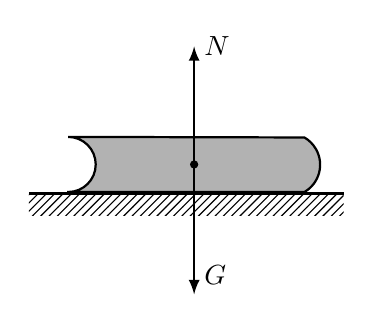
\begin{tikzpicture}[>=latex, thick,scale=1]
  % \useasboundingbox(-1,-0.75)rectangle(3.7,1.4);
  \fill [fill=black!30, draw,thick] (1,0.3)--(4,0.3)arc(-60:60:0.4)--(1,1)arc(90:-90:0.35)--cycle;
  \fill [pattern = north east lines] (0.5,0) rectangle (4.5,.28);
  \draw (0.5,.28)--(4.5,.28);
  \draw[->] (2.6,1.3/2)--(2.6, 1.3/2+1.5)node[right]{$N$};
  \draw[->] (2.6,1.3/2)--(2.6, 1.0/2-1.5)node[above right]{$G$};
  \fill (2.6,1.3/2) circle[radius=1.5pt];
\end{tikzpicture}
\end{document}